\chapter{Implementazione Hardware}
\label{chap:implementazione_hardware}
\section{Tecnologie di base}

In questo capitolo tratteremo tutte le tecnologie utilizzate nel progetto, come i microcontrollori e i dispositivi di output,
 concentrandoci sull’ESP32.

\subsection{Panoramica dell’ESP32}

\subsubsection{Generalità}
I microcontrollori (MCU) sono circuiti integrati che combinano nello stesso chip un microprocessore con una serie di componenti periferici
 come: memoria, timer, convertitori analogico-digitali e soprattutto pin di I/O.

A differenza di un microprocessore (CPU), i microcontrollori non sono pensati per svolgere onerose attività di calcolo ma per interagire 
il più possibile con l’ambiente esterno, gestendo numerosi scambi fra le periferiche di Input/Output.

L’ESP32, sviluppato da Espressif Systems, rappresenta un microcontrollore avanzato con architettura dual-core Tensilica LX6 a 32 bit
 (alcune varianti hanno anche core single-core o LX7), integrando al suo interno Wi-Fi e Bluetooth a basso consumo. Questa caratteristica
  lo rende particolarmente adatto per applicazioni IoT (Internet of Things), domotica e sistemi embedded complessi (Espressif, 2024 \cite{Espressif2024}).

\subsubsection{Famiglie di ESP32}
I microcontrollori sono suddivisi in famiglie a seconda del processore e delle periferiche integrate. Nel caso dell’ESP32,
 troviamo diverse varianti come ESP32-WROOM-32, ESP32-WROVER, ESP32-C3, ESP32-S2 ed ESP32-S3.  
Queste versioni condividono la stessa architettura di base ma differiscono per risorse di memoria, numero di GPIO disponibili,
 supporto a periferiche aggiuntive o funzionalità avanzate come acceleratori AI.  

La scelta del modulo da utilizzare deve essere fatta non sulla base delle prestazioni massime, ma dell’ottimalità rispetto al
 progetto in questione (Patti, 2024 \cite{Patti2024}).

\subsubsection{Componenti hardware}
Ogni ESP32 integra al suo interno non solo la CPU, ma anche le memorie e una grande quantità di periferiche digitali e analogiche, 
oltre ai moduli di comunicazione wireless (Wi-Fi 802.11 b/g/n e Bluetooth 4.2/5.0).  
Questa elevata integrazione consente di ridurre i costi, semplificare il design e garantire maggiore velocità di accesso ai dati.

\begin{figure}[H]
\centering
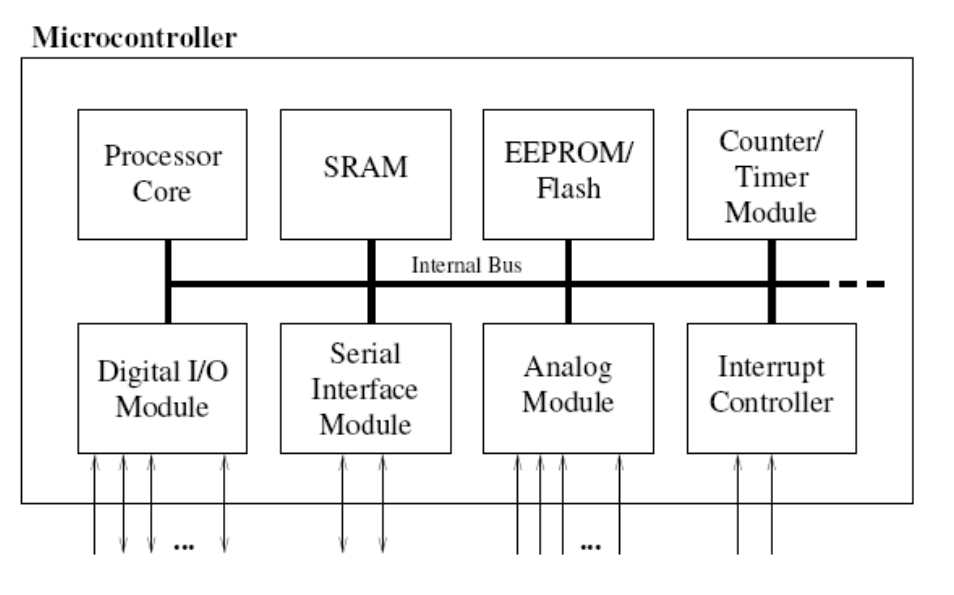
\includegraphics[width=0.7\textwidth]{esp32_block_diagram.png}
\caption{Componenti hardware principali di un microcontrollore ESP32.}
\label{fig:esp32-mcu}
\end{figure}

\subsubsection{Memorie}
Le memorie di un microcontrollore possono essere di tipo volatile e non volatile. Le volatili includono SRAM e DRAM; le non volatili comprendono ROM, EEPROM, Flash e, in alcuni casi, NVRAM.

L’ESP32 tipicamente dispone di:
\begin{itemize}
    \item 448 KB di ROM, che contiene il bootloader e alcune librerie di base;
    \item 520 KB di SRAM interna, divisa tra cache, stack e heap per le applicazioni;
    \item Flash esterna fino a 16 MB (a seconda del modulo), utilizzata per memorizzare codice e file system;
    \item opzionalmente, PSRAM esterna fino a 8 MB, utile per applicazioni che richiedono elaborazioni multimediali o server web embedded.
\end{itemize}

Rispetto ad altre schede, l’ESP32 si distingue per la disponibilità di memoria e per la presenza di connettività wireless integrata, rendendolo una soluzione più completa per progetti IoT e sistemi embedded avanzati (Patti, 2024 \cite{Patti2024}; Espressif, 2024 \cite{Espressif2024}).

\subsection{Periferiche di Input/Output}
Le periferiche di Input/Output (I/O) sono componenti essenziali che permettono al microcontrollore di interagire con il mondo esterno.
Per la realizzazione del progetto sono state utilizzate diverse periferiche, in questa sezione se ne approfondiscono le loro caratteristiche.\\
\noindent
Tutta la componentistica impiegata in questo progetto è stata selezionata dal catalogo \textbf{Adafruit Industries}. 
La scelta è motivata dall'elevata qualità dei loro moduli, dalla cura del layout dei circuiti stampati e dalla ricca documentazione tecnica a corredo, che garantiscono affidabilità in fase di prototipazione e semplicità di integrazione. 
L'utilizzo di componenti a marchio Adafruit riduce i rischi di incompatibilità o malfunzionamenti tipici dei cloni economici e assicura un supporto didattico di livello professionale.


\subsubsection{Microfono MEMS I2S digitale Adafruit -- SPH0645LM4H}
\label{subsec:mic}
Il breakout Adafruit (cod. 3421) monta il microfono MEMS digitale \textbf{Knowles SPH0645LM4H-B}, bottom–port, con uscita \textbf{I$^2$S} \cite{adafruit-guide,adafruit-product}. 
È un dispositivo \emph{slave} che richiede dal master le linee di clock (\texttt{BCLK}, \texttt{LRCLK}) \cite{nordic-devzone}. 
Fornisce direttamente campioni PCM a 24 bit (con 18 bit effettivi), evitando stadi analogici esterni \cite{knowles-datasheet}.
\begin{figure}[H]
  \centering
  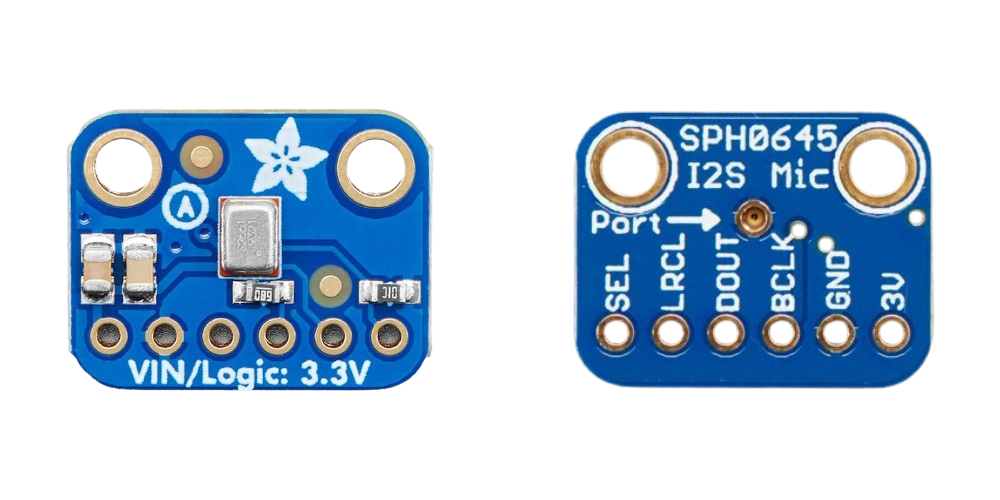
\includegraphics[width=0.7\textwidth]{adafruit_mems.png}
  \caption{Microfono MEMS I2S digitale Adafruit SPH0645LM4H-B.}
  \label{fig:adafruit_mems}
  \end{figure}

\paragraph{Caratteristiche principali.}
\begin{itemize}
  \item Alimentazione: \SIrange{1.62}{3.6}{V}, logica \SI{3.3}{V}, tipico consumo \SI{600}{\micro A} \cite{digikey-sheet}.
  \item Interfaccia: I$^2$S, pin \texttt{BCLK}, \texttt{LRCLK}, \texttt{DOUT}, \texttt{SEL}, più \texttt{3V} e \texttt{GND}.
  \item Formato dati: parole a 24 bit (MSB first, complemento a due), 18 bit utili, oversampling ratio (OSR) = 64 \cite{knowles-datasheet}.
  \item Prestazioni: SNR tip. \SI{65}{dB(A)}, AOP \SI{120}{dB\,SPL}, sensibilità $\sim -26$ dBFS @ \SI{94}{dB\,SPL} \cite{knowles-datasheet}.
\end{itemize}

\paragraph{Pinout e collegamenti.} 
Due moduli possono essere usati in stereo condividendo \texttt{BCLK}, \texttt{LRCLK}, \texttt{DOUT}; \texttt{SEL} basso/alto definisce L/R. 
In modalità mono basta un solo modulo con \texttt{SEL} a GND (Left di default) \cite{adafruit-guide}.

\paragraph{Interfaccia I$^2$S.} 
Il microfono trasmette in formato \emph{Philips}: ogni semiperiodo di \texttt{LRCLK} contiene una parola da 24 bit. 
La relazione fondamentale è $\mathrm{BCLK}=64f_s$ \cite{nordic-devzone}. 
Tipici: \SI{3.072}{MHz} per \SI{48}{kHz}, \SI{2.8224}{MHz} per \SI{44.1}{kHz}.

\paragraph{Catena del segnale interna.}
\begin{enumerate}
  \item Trasduttore MEMS capacitivo: diaframma + backplate $\to$ capacità $C(t)$.
  \item Amplificatore a carica: traduce $\Delta C$ in tensione.
  \item Modulatore $\Sigma\Delta$: noise–shaping fuori banda audio.
  \item Filtro di decimazione: riduce a $f_s$ mantenendo 18 bit effettivi.
  \item Serializer: prepara le parole I$^2$S.
\end{enumerate}

\paragraph{Fondamenti fisici.}
La pressione $p(t)$ agisce sul diaframma (massa $m$, molla $k$, smorzamento $b$) \cite{mems-acoustics}:
\[
m\ddot{x}+b\dot{x}+kx=S\,p(t)
\]
La variazione di capacità è $\Delta C/C_0 \approx x/d_0$, con risonanza a $\omega_0=\sqrt{k/m}$. 
Il rumore complessivo deriva da contributi termico–meccanici, elettronici e quantizzazione. 
Il back–volume e la porta acustica modellano la risposta in frequenza (roll–off alle basse, ondulazioni agli alti) \cite{mems-acoustics}.
\begin{figure}[H]
  \centering
  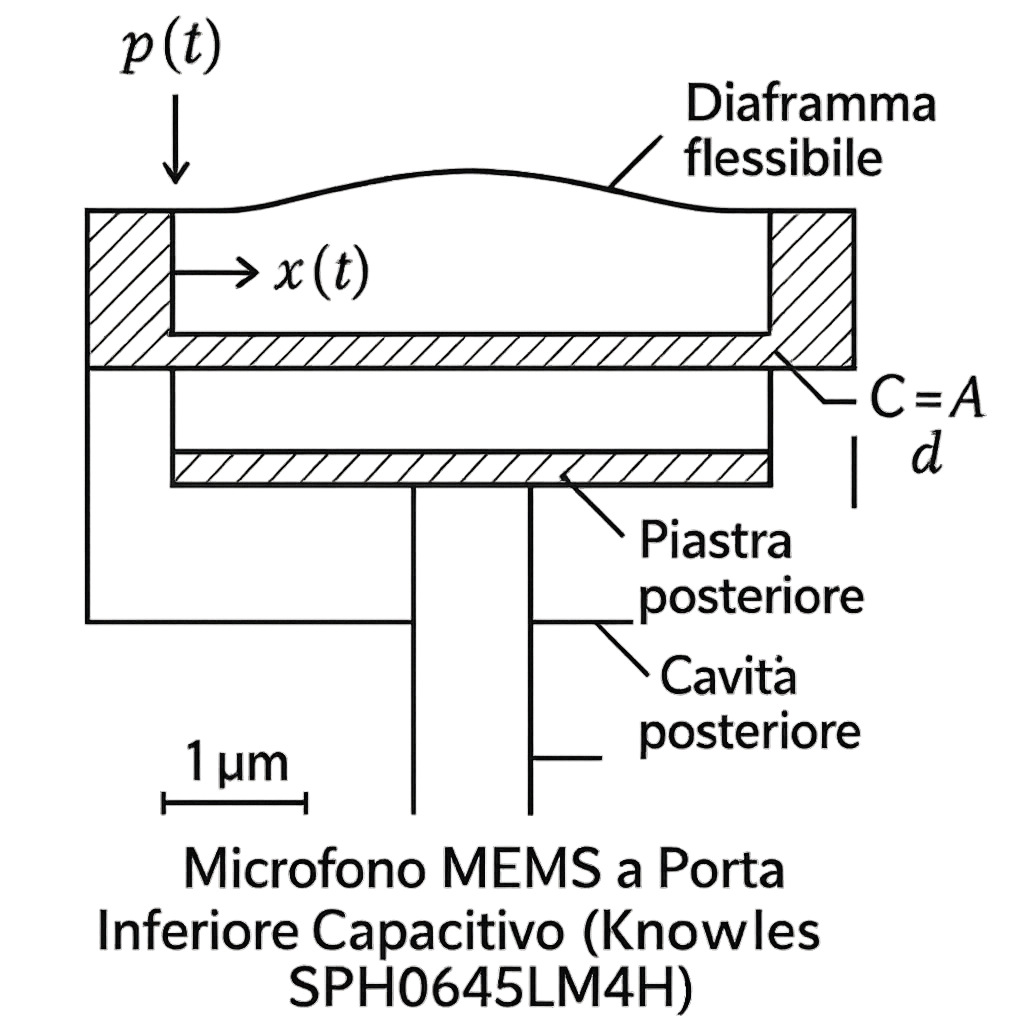
\includegraphics[width=0.4\textwidth]{adafruit_diaframma.png}
  \caption{Sezione verticale del microfono Adafruit MEMS.}
  \label{fig:adafruit_diaframma}
  \end{figure}

\paragraph{Limiti.} Non tollera \SI{5}{V}, banda garantita $\sim$\SI{20}{Hz}--\SI{10}{kHz} (utilizzabile fino a $\sim$\SI{15}{kHz} secondo Adafruit) \cite{adafruit-product}, OSR fisso (meno flessibile di PDM).

\paragraph{Relazione dBFS--SPL.}
\SI{94}{dB\,SPL} = \SI{1}{Pa} $\Rightarrow$ $\approx -26$ dBFS RMS \cite{knowles-datasheet}. 
L’AOP a \SI{120}{dB\,SPL} ($\sim$\SI{20}{Pa}) indica il massimo senza distorsione significativa.


\subsubsection{Adafruit MAX98357A I$^2$S Amplificatore Classe-D}

Il breakout Adafruit basato sul chip \textbf{MAX98357A} è un amplificatore audio digitale in classe D, in grado di convertire direttamente un flusso
 I$^2$S in segnale audio analogico amplificato per pilotare altoparlanti a bassa impedenza. 
La caratteristica principale è l’eliminazione della necessità di un DAC esterno: il MAX98357A integra al suo interno la conversione digitale-analogica, 
il filtraggio, e la sezione di potenza \cite{maxim-datasheet,adafruit-guide-max98357}.
\begin{figure}[H]
  \centering
  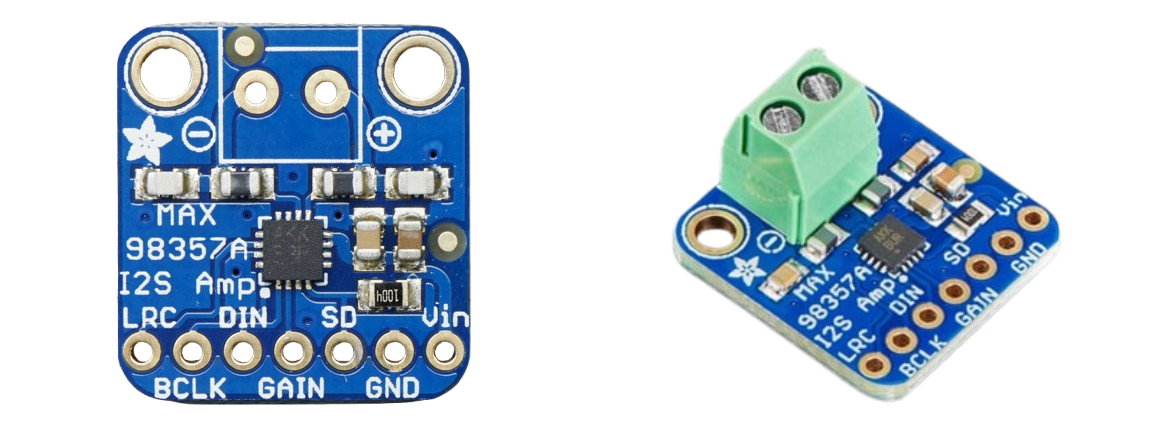
\includegraphics[width=0.7\textwidth]{adafruit_max.png}
  \caption{Amplificatore digitale Classe-D Adafruit MAX98357A.}
  \label{fig:adafruit_max}
  \end{figure}
\paragraph{Caratteristiche essenziali.}
\begin{itemize}
  \item \textbf{Alimentazione}: \SIrange{2.5}{5.5}{V}, con tensione tipica \SI{3.3}{V} o \SI{5}{V}. 
  \item \textbf{Potenza d’uscita}: fino a \SI{3.2}{W} su \SI{4}{\ohm} a \SI{5}{V}, THD+N $\approx$ \SI{1}{\%}.
  \item \textbf{Interfaccia}: I$^2$S standard (\texttt{BCLK}, \texttt{LRCLK}, \texttt{DIN}); pin aggiuntivi per modalità (\texttt{GAIN}, \texttt{SD}, \texttt{DMP}).
  \item \textbf{Efficienza}: superiore all’$\SI{85}{\%}$ grazie all’architettura in classe D.
  \item \textbf{Gamma dinamica}: $\approx \SI{98}{dB}$, con rumore di fondo contenuto \cite{maxim-datasheet}.
\end{itemize}

\paragraph{Funzionamento.}
Il MAX98357A riceve un flusso I$^2$S in formato PCM (\SI{16}{}, \SI{24}{} o \SI{32}{bit}, standard Philips). L’architettura interna comprende:
\begin{enumerate}
  \item \textbf{Interfaccia I$^2$S}: decodifica il flusso digitale e gestisce il framing (left/right).
  \item \textbf{DAC sigma–delta}: converte i campioni PCM in una modulazione a densità di impulsi.
  \item \textbf{Driver in classe D}: due MOSFET push-pull pilotano direttamente l’altoparlante in configurazione \emph{bridge-tied load (BTL)}.
  \item \textbf{Filtro LC virtuale}: la stessa induttanza del carico acustico e la risposta del driver fungono da filtro passa-basso, eliminando la componente PWM ad alta frequenza.
\end{enumerate}
\begin{figure}[H]
  \centering
  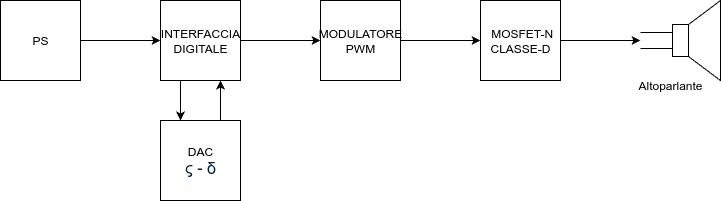
\includegraphics[width=0.7\textwidth]{max_diagram.png}
  \caption{Funzionamento interno del MAX98357A.}
  \label{fig:max_diagram}
  \end{figure}
\paragraph{Motivazioni fisiche del funzionamento.}
L’amplificatore in classe D si basa su modulazione a \emph{duty cycle} dei MOSFET: il segnale analogico ricostruito corrisponde al valore medio del PWM. L’elevata efficienza deriva dal fatto che i transistor lavorano quasi sempre in saturazione o interdizione, riducendo le perdite per dissipazione. L’integrazione del DAC sigma–delta consente un noise-shaping che sposta il rumore di quantizzazione fuori banda audio, garantendo un’ottima qualità percepita \cite{texas-classd}.

\section{Progettazione digitale}
Per la progettazione digitale del sistema è stato utilizzato il software \textbf{Fritzing}, un tool open-source
per la progettazione di circuiti elettronici, con la possibilità di creare moduli personaizzati.\\
Nel capito \ref{chap:design_protocollo} è stato descritto il protocollo di comunicazione, facendo riferimento al \textbf{Livello Fisico},
come il livello più basso del modello. L'interazione I/O con il mondo circostante che avviene nel Livello Fisico, è realizzata con due componenti: una software, 
che tratteremo a breve nel capitolo \ref{chap:implementazione_software}, e una hardware, che vedremo in questo capitolo.\\
Il Livello Fisico è realizzato con due periferiche di Input/Output, il microfono MEMS digitale e l'amplificatore Classe-D, che comunicano con il microcontrollore ESP32
 tramite il protocollo I$^2$S.\\

Per la realizzazione del circuito elettronico sono stati utilizzati due breakout board Adafruit, che integrano i componenti necessari per il corretto funzionamento
  del microfono e dell'amplificatore.\\
  L'utilizzo del microfono MEMS I2S digitale Adafruit SPH0645LM4H viene da una selezione accurata, basata su test di qualità,
  il progetto, che all'inizio prevedeva un microfono analogico, è stato modificato per utilizzare un microfono digitale,
  in quanto i test effettuati con il microfono analogico non hanno dato risultati soddisfacenti.\\



  \subsection{Collegamento del microfono digitale I$^2$S}
  \label{subsec:conn_mic}
  
  La \autoref{fig:board_microfono} mostra lo schema di cablaggio realizzato in \textbf{Fritzing} tra la breakout Adafruit basata sul microfono MEMS digitale \textbf{SPH0645LM4H} e la \textbf{ESP32}, mediante il bus \textbf{I$^2$S} (Inter-IC Sound). L’interfaccia prevede tre linee digitali di segnale
  (BCLK, LRCLK, DOUT) e due linee di alimentazione (3V3, GND), oltre al pin SEL per la selezione del canale logico (sinistro/destro).
  
  \begin{figure}[H]
    \centering
    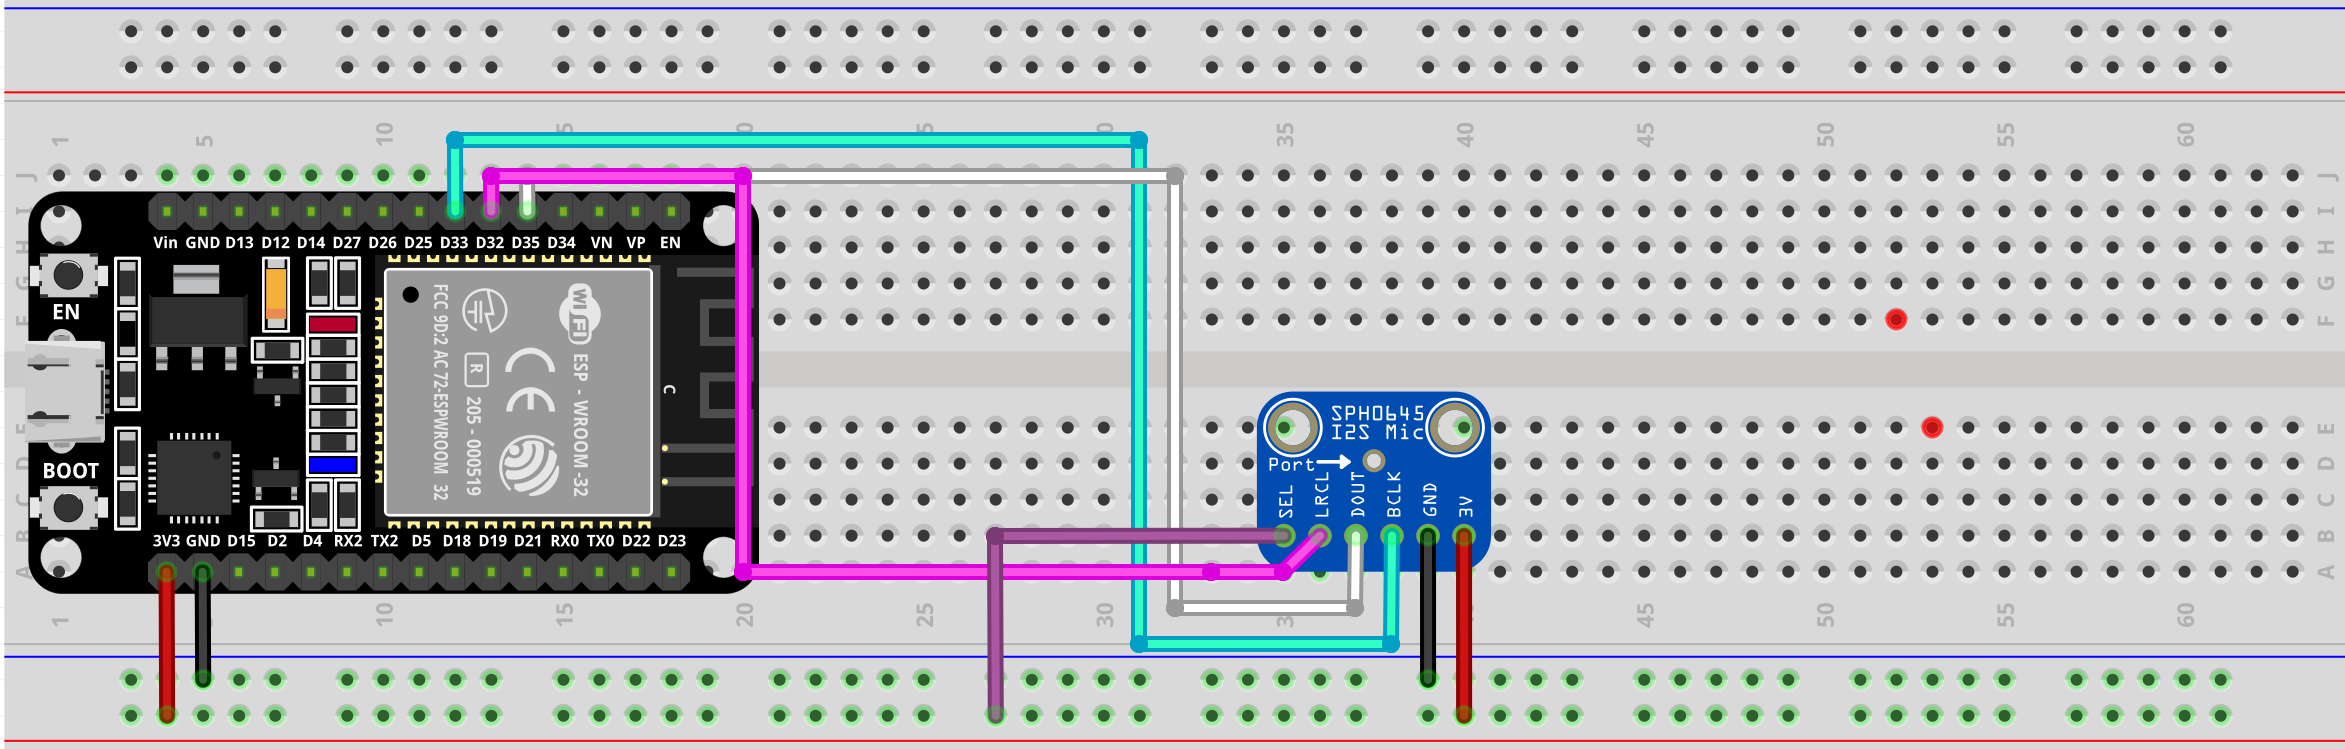
\includegraphics[width=\textwidth]{board_microfono.png}
    \caption{Collegamento fisico tra ESP32 e microfono I$^2$S (Adafruit SPH0645LM4H) su breadboard.}
    \label{fig:board_microfono}
  \end{figure} 

  \paragraph{Pinout del modulo microfonico.}
  Sulla scheda Adafruit, da sinistra a destra (come serigrafato) sono presenti i pin: SEL, LRCL (o LRCLK/WS), DOUT (o SD), BCLK (o SCK), GND, 3V.  
  DOUT è un’uscita a logica \SI{3.3}{\volt}; LRCLK e BCLK sono ingressi di clock; SEL è un ingresso statico per selezionare su quale slot (sinistro o destro) il microfono presenta i campioni sul bus I$^2$S.
  
  \paragraph{Mappatura dei segnali sull'ESP32.}
  La Tab.~\ref{tab:i2s_pins} riassume la corrispondenza dei pin usati, come nella figura. Le scelte rispettano i vincoli dell'ESP32 (evitando pin con funzioni di strapping all'avvio come GPIO15-12 o limitazioni di sola-lettura).
  
  \definecolor{lightgray}{RGB}{235,235,235}
  \definecolor{white}{RGB}{255,255,255}
  
  \begin{table}[H]
    \centering
    \label{tab:i2s_pins}
    \resizebox{\textwidth}{!}{%
    \begin{tabular}{|l|>{\columncolor{lightgray}}l|l|>{\columncolor{lightgray}}l|}
      \hline
    
      \textbf{Pin modulo} & \textbf{Segnale} & \textbf{Pin ESP32 (sigla serigrafata)} \\
      \hline
    
      3V   & Alimentazione \SI{3.3}{\volt}       & 3V3 \\
      \hline
    
      GND  & Riferimento di massa                & GND \\
      \hline
    
      BCLK & Bit Clock I$^2$S                    & GPIO14 (D14) \\
      \hline
    
      LRCL & Word-Select / LRCLK                 & GPIO25 (D25) \\
      \hline
    
      DOUT & Serial Data (uscita microfono)      & GPIO32 (D32) \\
      \hline
    
      SEL  & Selezione canale                    & GND $\rightarrow$ canale sinistro\\
      \hline
    
    \end{tabular}
    
    }
    \caption{Mappatura hardware dei pin I$^2$S tra ESP32 e microfono SPH0645LM4H.}
  
  \end{table}
  
  \noindent
  Il segnale SEL determina in quale slot vengono emessi i campioni audio: se portato a massa (SEL = GND) i dati escono sul canale sinistro,
  mentre a livello alto (SEL = 3V3) sul destro. \\
  Nel nostro schema è stato fissato a 3V3, quindi l’uscita è forzata a destra.
  Questo a seguito di alcuni test dove si è verificato che per qualche difformita nel IC il canale destro garantiva maggiore precisione.\\
  
  \paragraph{Dettagli elettrici e motivazioni delle scelte.}
  Il microfono Adafruit SPH0645LM4H funziona solo a 3.3 V: non sono previsti level shifter e un’alimentazione a 5 V lo danneggerebbe \cite{digikey-sheet}. L’assorbimento è dell’ordine dei mA, quindi l’uscita 3V3 dell’ESP32 è più che sufficiente \cite{digikey-sheet}.
    
  Per l’ESP32 si è scelto \textbf{GPIO14 come BCLK, GPIO25 come LRCLK e GPIO32} per il dato in ingresso.
    
  Infine, il microfono trasmette campioni a 24 bit allineati su frame da 32 come discusso precedentemente nella sezione \ref{subsec:mic}.
  
 
\subsection{Collegamento dell’amplificatore digitale I$^2$S}
\label{subsec:conn_amp}

La \autoref{fig:board_amp} mostra lo schema di cablaggio realizzato in \textbf{Fritzing} tra la breakout Adafruit basata sul chip \textbf{MAX98357A}
 (amplificatore in classe D con interfaccia I$^2$S) e la \textbf{ESP32}.  
L’interfaccia prevede tre linee digitali di segnale
(BCLK, LRCLK, DIN) e due linee di alimentazione (3V3, GND). Il modulo espone inoltre i pin di configurazione \textbf{GAIN} e \textbf{SD} (shutdown), 
che in questo caso non vengono utilizzati e restano flottanti.

\begin{figure}[H]
  \centering
  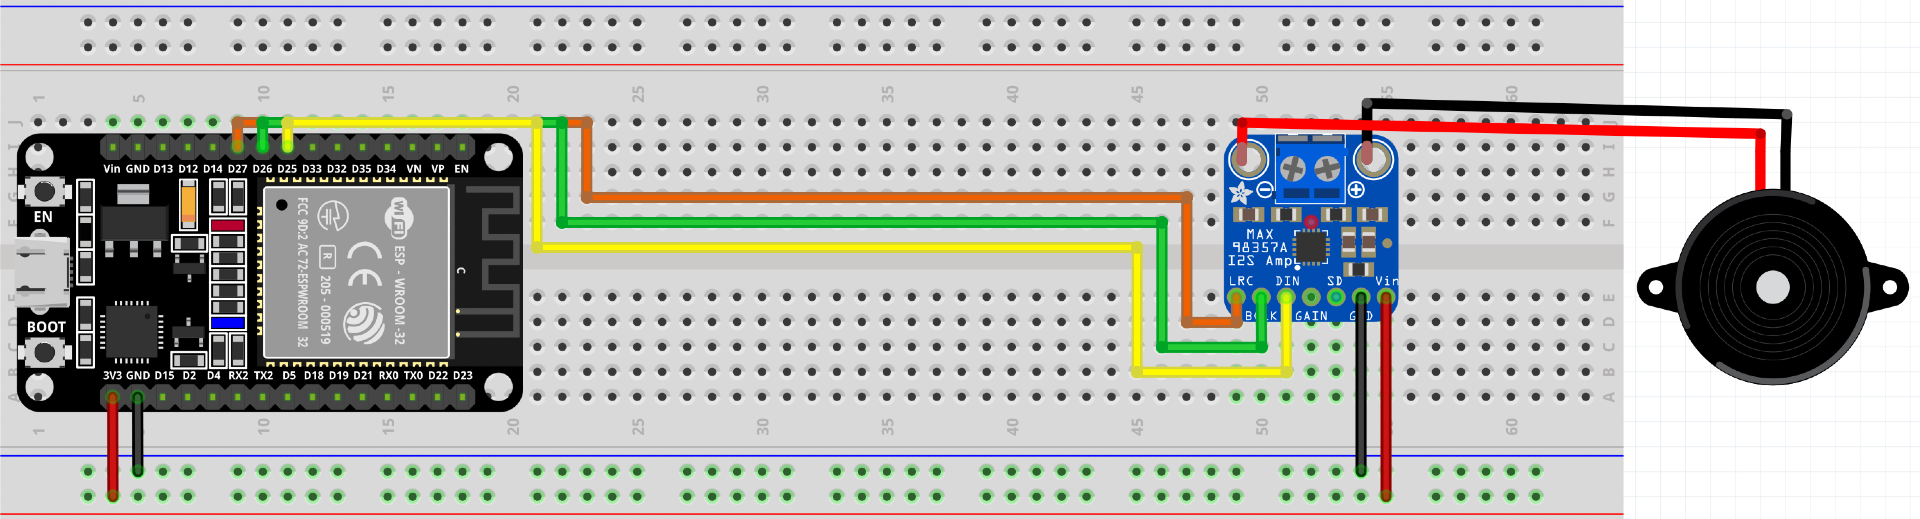
\includegraphics[width=\textwidth]{board_amp.png}
  \caption{Collegamento fisico tra ESP32 e amplificatore I$^2$S (Adafruit MAX98357A) su breadboard.}
  \label{fig:board_amp}
\end{figure} 

\paragraph{Pinout del modulo amplificatore.}
Sulla scheda Adafruit, da sinistra a destra (come serigrafato) sono presenti i pin: GAIN, SD, DIN, BCLK, LRCLK, GND, Vin.  
Il pin \textbf{DIN} è l’ingresso dati audio seriali (logica \SI{3.3}{\volt}); \textbf{BCLK} e \textbf{LRCLK} sono segnali di clock forniti dall’ESP32; \textbf{Vin} riceve l’alimentazione (3–5 V, compatibile col regolatore onboard).  
I pin GAIN e SD sono opzionali: GAIN permette di configurare il guadagno interno tramite resistenze, mentre SD forza il chip in modalità risparmio energetico.

\paragraph{Mappatura dei segnali sull'ESP32.}
La Tab.~\ref{tab:i2s_pins_amp} riassume la corrispondenza dei pin usati, come nello schema. Anche in questo caso la scelta dei GPIO tiene conto delle raccomandazioni di Espressif, evitando pin con funzioni critiche all’avvio.


\begin{table}[H]
  \centering
  \label{tab:i2s_pins_amp}
  \resizebox{\textwidth}{!}{%
  \begin{tabular}{|l|>{\columncolor{lightgray}}l|l|}
    \hline
  
    \textbf{Pin modulo} & \textbf{Segnale} & \textbf{Pin ESP32 (sigla serigrafata)} \\
    \hline
  
    Vin  & Alimentazione \SI{3.3}{\volt} / \SI{5}{\volt} & 3V3 \\
    \hline
  
    GND  & Riferimento di massa                        & GND \\
    \hline
  
    BCLK & Bit Clock I$^2$S                            & GPIO14 (D14) \\
    \hline
  
    LRCLK & Word-Select / LRCLK                        & GPIO25 (D25) \\
    \hline
  
    DIN  & Serial Data (ingresso audio)                & GPIO26 (D26) \\
    \hline
  
    SD   & Shutdown (non connesso)                     & -- \\
    \hline
  
    GAIN & Configurazione guadagno (non connesso)      & -- \\
    \hline
  
  \end{tabular}
  }
  \caption{Mappatura hardware dei pin I$^2$S tra ESP32 e amplificatore MAX98357A.}
\end{table}

\noindent
Il collegamento all’altoparlante avviene direttamente dai terminali di uscita del modulo (OUT$+$, OUT$-$), come mostrato in figura.  
Essendo un amplificatore in classe D capace di pilotare piccoli altoparlanti (4–8~$\Omega$, fino a circa \SI{3}{W} a 5 V),
 non è necessaria ulteriore elettronica per il collegamento all'altoparlante.

\paragraph{Dettagli elettrici e motivazioni delle scelte.}
Il MAX98357A accetta alimentazione sia a 3.3 V che a 5 V \cite{maxim-datasheet}: in questo schema si è scelto di usare il \textbf{3V3 dell’ESP32} per semplicità,
 tenendo conto che ciò limita la potenza massima erogabile all’altoparlante e considerando che in
  una reale applicazione a scopo industriale si utilizzerebbero amplificatori da \~ 230 V.  
Il consumo è nell’ordine di poche decine di mA a volume medio, quindi l’uscita 3V3 dell’ESP32 è sufficiente in prototipazione.  



\subsection{Sistema di segnalazione LED}
\label{subsec:led_system}

La \autoref{fig:board_led} mostra lo schema di cablaggio realizzato in \textbf{Fritzing} tra la scheda \textbf{ESP32} e tre LED collegati su breadboard.  
Il sistema fornisce un feedback visivo sullo stato di decodifica del segnale audio, a supporto del protocollo discusso nella sezione \ref{sec:filtraggio}.  

\begin{figure}[H]
  \centering
  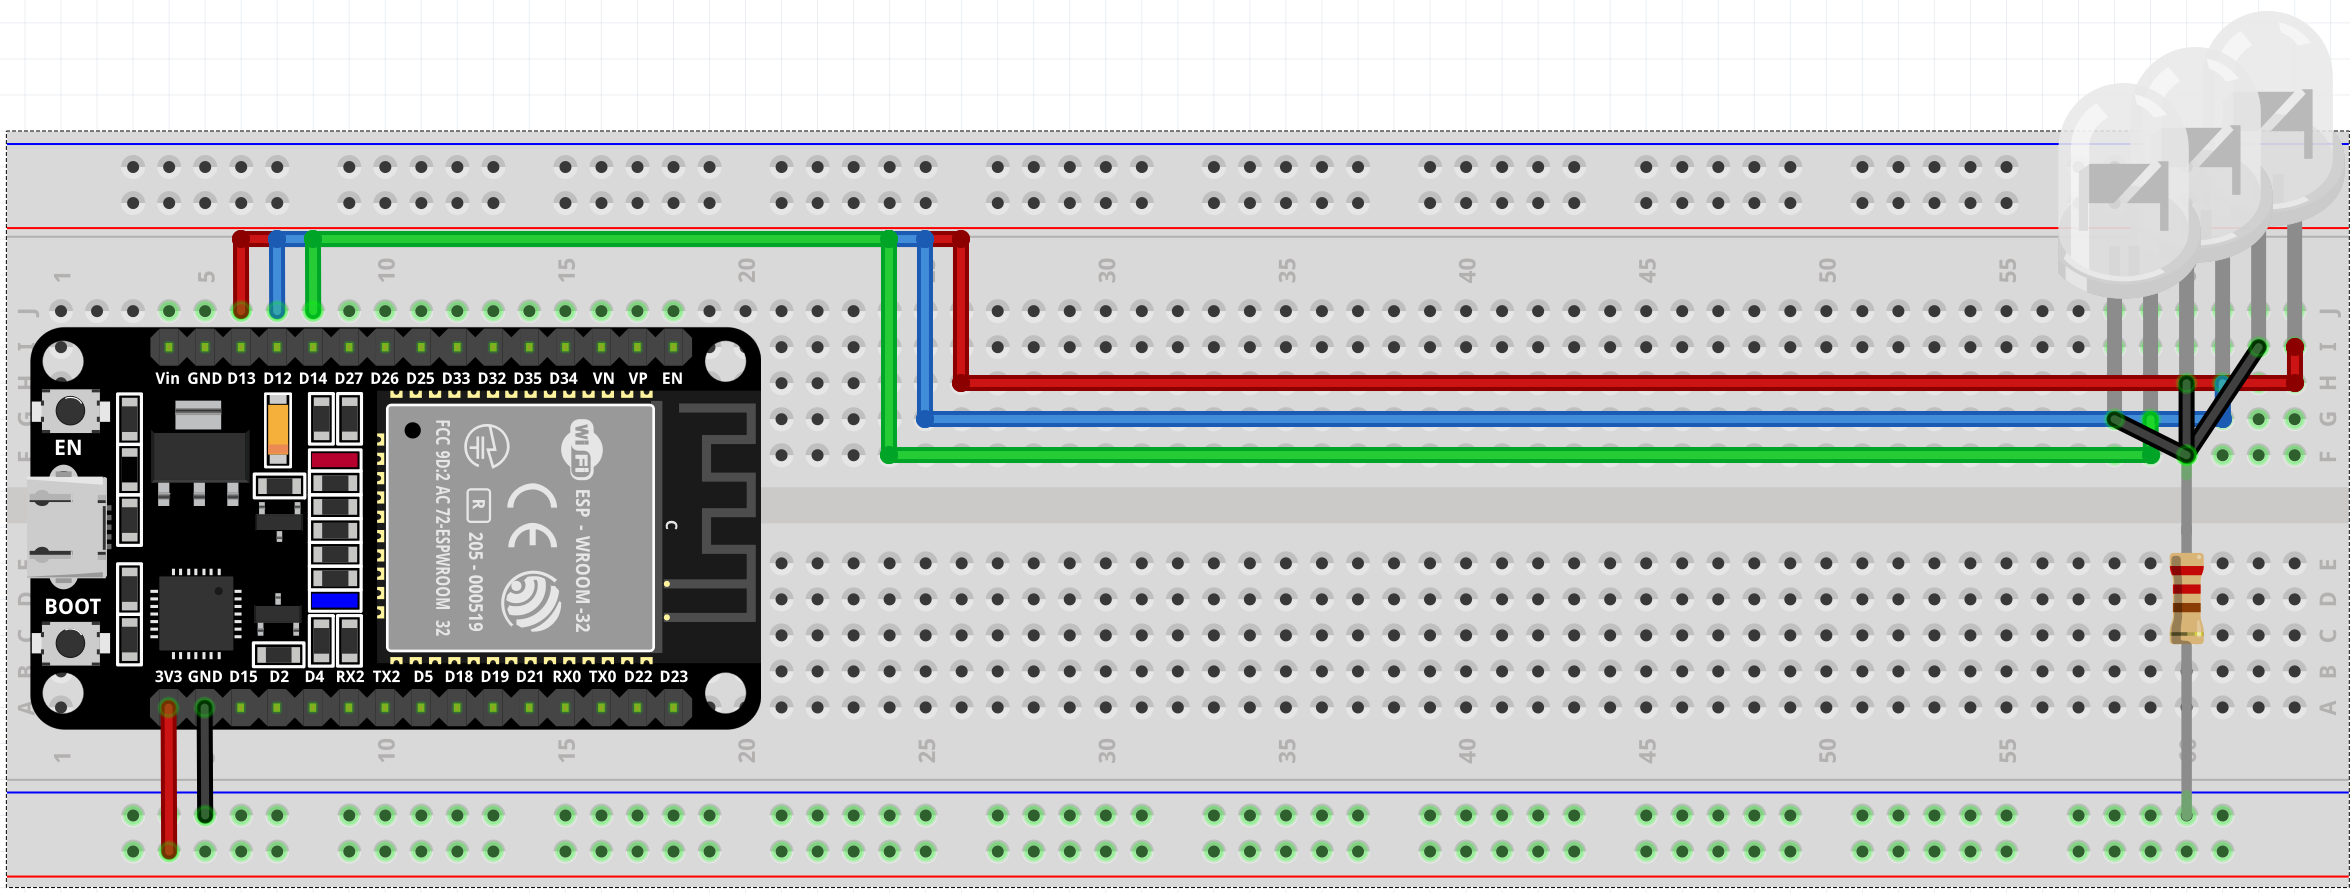
\includegraphics[width=\textwidth]{board_led.png}
  \caption{Collegamento fisico tra ESP32 e LED di segnalazione su breadboard.}
  \label{fig:board_led}
\end{figure} 

\paragraph{Funzionamento del sistema.}
Sono stati utilizzati tre LED di colore diverso (verde, blu e rosso) per rappresentare in modo immediato lo stato di elaborazione:  
\begin{itemize}
  \item LED verde: il segnale è stato decodificato correttamente;
  \item LED blu: il segnale è in fase di decodifica;
  \item LED rosso: il segnale non ha superato il controllo dell’interpolazione parabolica e non è stato decodificato correttamente.
\end{itemize}

\paragraph{Mappatura dei segnali sull'ESP32.}
La Tab.~\ref{tab:led_pins} riassume la corrispondenza dei pin usati per il pilotaggio dei tre LED, come nello schema in figura.  
Ogni LED è collegato in serie a una resistenza di limitazione, necessaria a ridurre la corrente entro i limiti di sicurezza per i GPIO dell’ESP32 (massimo \SI{12}{mA} consigliati).

\definecolor{lightgray}{RGB}{235,235,235}
\definecolor{white}{RGB}{255,255,255}

\begin{table}[H]
  \centering
  \label{tab:led_pins}
  \resizebox{\textwidth}{!}{%
  \begin{tabular}{|l|>{\columncolor{lightgray}}l|l|}
    \hline
  
    \textbf{LED} & \textbf{Funzione} & \textbf{Pin ESP32 (sigla serigrafata)} \\
    \hline
  
    Verde & Decodifica corretta & GPIO14 (D14) \\
    \hline
  
    Blu   & Decodifica in corso & GPIO27 (D27) \\
    \hline
  
    Rosso & Errore di decodifica & GPIO26 (D26) \\
    \hline
  
  \end{tabular}
  }
  \caption{Mappatura hardware dei pin di uscita dell’ESP32 verso i LED di stato.}
\end{table}

\paragraph{Dettagli elettrici e motivazioni delle scelte.}
Ciascun LED è collegato al rispettivo GPIO tramite una resistenza da \SI{220}{\ohm}, sufficiente a limitare la corrente senza ridurre eccessivamente la luminosità.  
I pin \textbf{GPIO14, GPIO27 e GPIO26} sono stati scelti in quanto liberi da vincoli di boot e comunemente usati per uscite digitali.  

\subsection{Bottone di Hotspot}
\label{subsec:button_hotspot}

La \autoref{fig:board_bottone} mostra il collegamento su breadboard di un pulsante e due LED all’ESP32.  
Il pulsante è collegato al pin \textbf{GPIO34 (D34)} e consente di abilitare la modalità \textit{hotspot} prevista dal protocollo (\ref{sec:livello_link}).  

\begin{figure}[H]
  \centering
  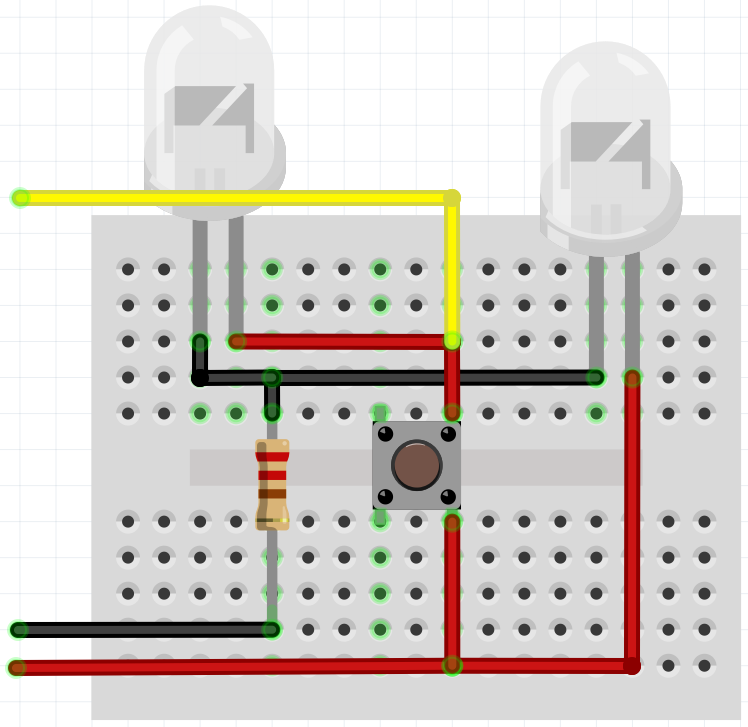
\includegraphics[width=0.35\textwidth]{board_bottone.png}
  \caption{Schema di collegamento del bottone e dei LED di stato per la modalità hotspot.}
  \label{fig:board_bottone}
\end{figure}

Il LED giallo, a sinistra, indica l’attivazione dell’hotspot e si accende solo alla pressione del pulsante.  
Il LED a destra segnala invece lo stato di alimentazione della scheda, acceso quando l’ESP32 è in funzione e spento in assenza di alimentazione.  
 
\subsection{Circuito completo}
\label{subsec:circuito_completo}

La \autoref{fig:board_completa} riassume l’intero sistema realizzato su breadboard, integrando in un 
unico schema tutte le funzionalità descritte nelle sezioni precedenti. L’\textbf{ESP32}, alimentato da 
un pacco batterie AAA, costituisce il cuore del circuito e gestisce sia la parte di acquisizione sia quella 
di elaborazione e segnalazione. \\
Il microfono \textbf{I²S} raccoglie il segnale audio e lo invia al microcontrollore, 
che a sua volta lo riproduce attraverso l’amplificatore digitale \textbf{MAX98357A} collegato a un piccolo altoparlante.\\
 In parallelo, il sistema integra un’interfaccia visiva con tre LED che indicano lo stato della decodifica, insieme a un
  pulsante dedicato all’attivazione della modalità \textit{hotspot}, il cui stato è reso evidente da un ulteriore LED giallo. \\
  Tutti i collegamenti sono realizzati su breadboard, con le linee di alimentazione distribuite ai vari moduli e i segnali instradati 
  verso i pin dell’ESP32, tra cui il \textbf{GPIO34}, correttamente utilizzato come ingresso per il pulsante. In questo modo il circuito 
  offre un esempio completo di integrazione tra acquisizione, elaborazione, riproduzione e interfaccia utente, consentendo il passaggio 
  fluido dall’ascolto alla decodifica, fino alla segnalazione visiva e al controllo della connessione wireless.

\begin{figure}[H]
  \centering
  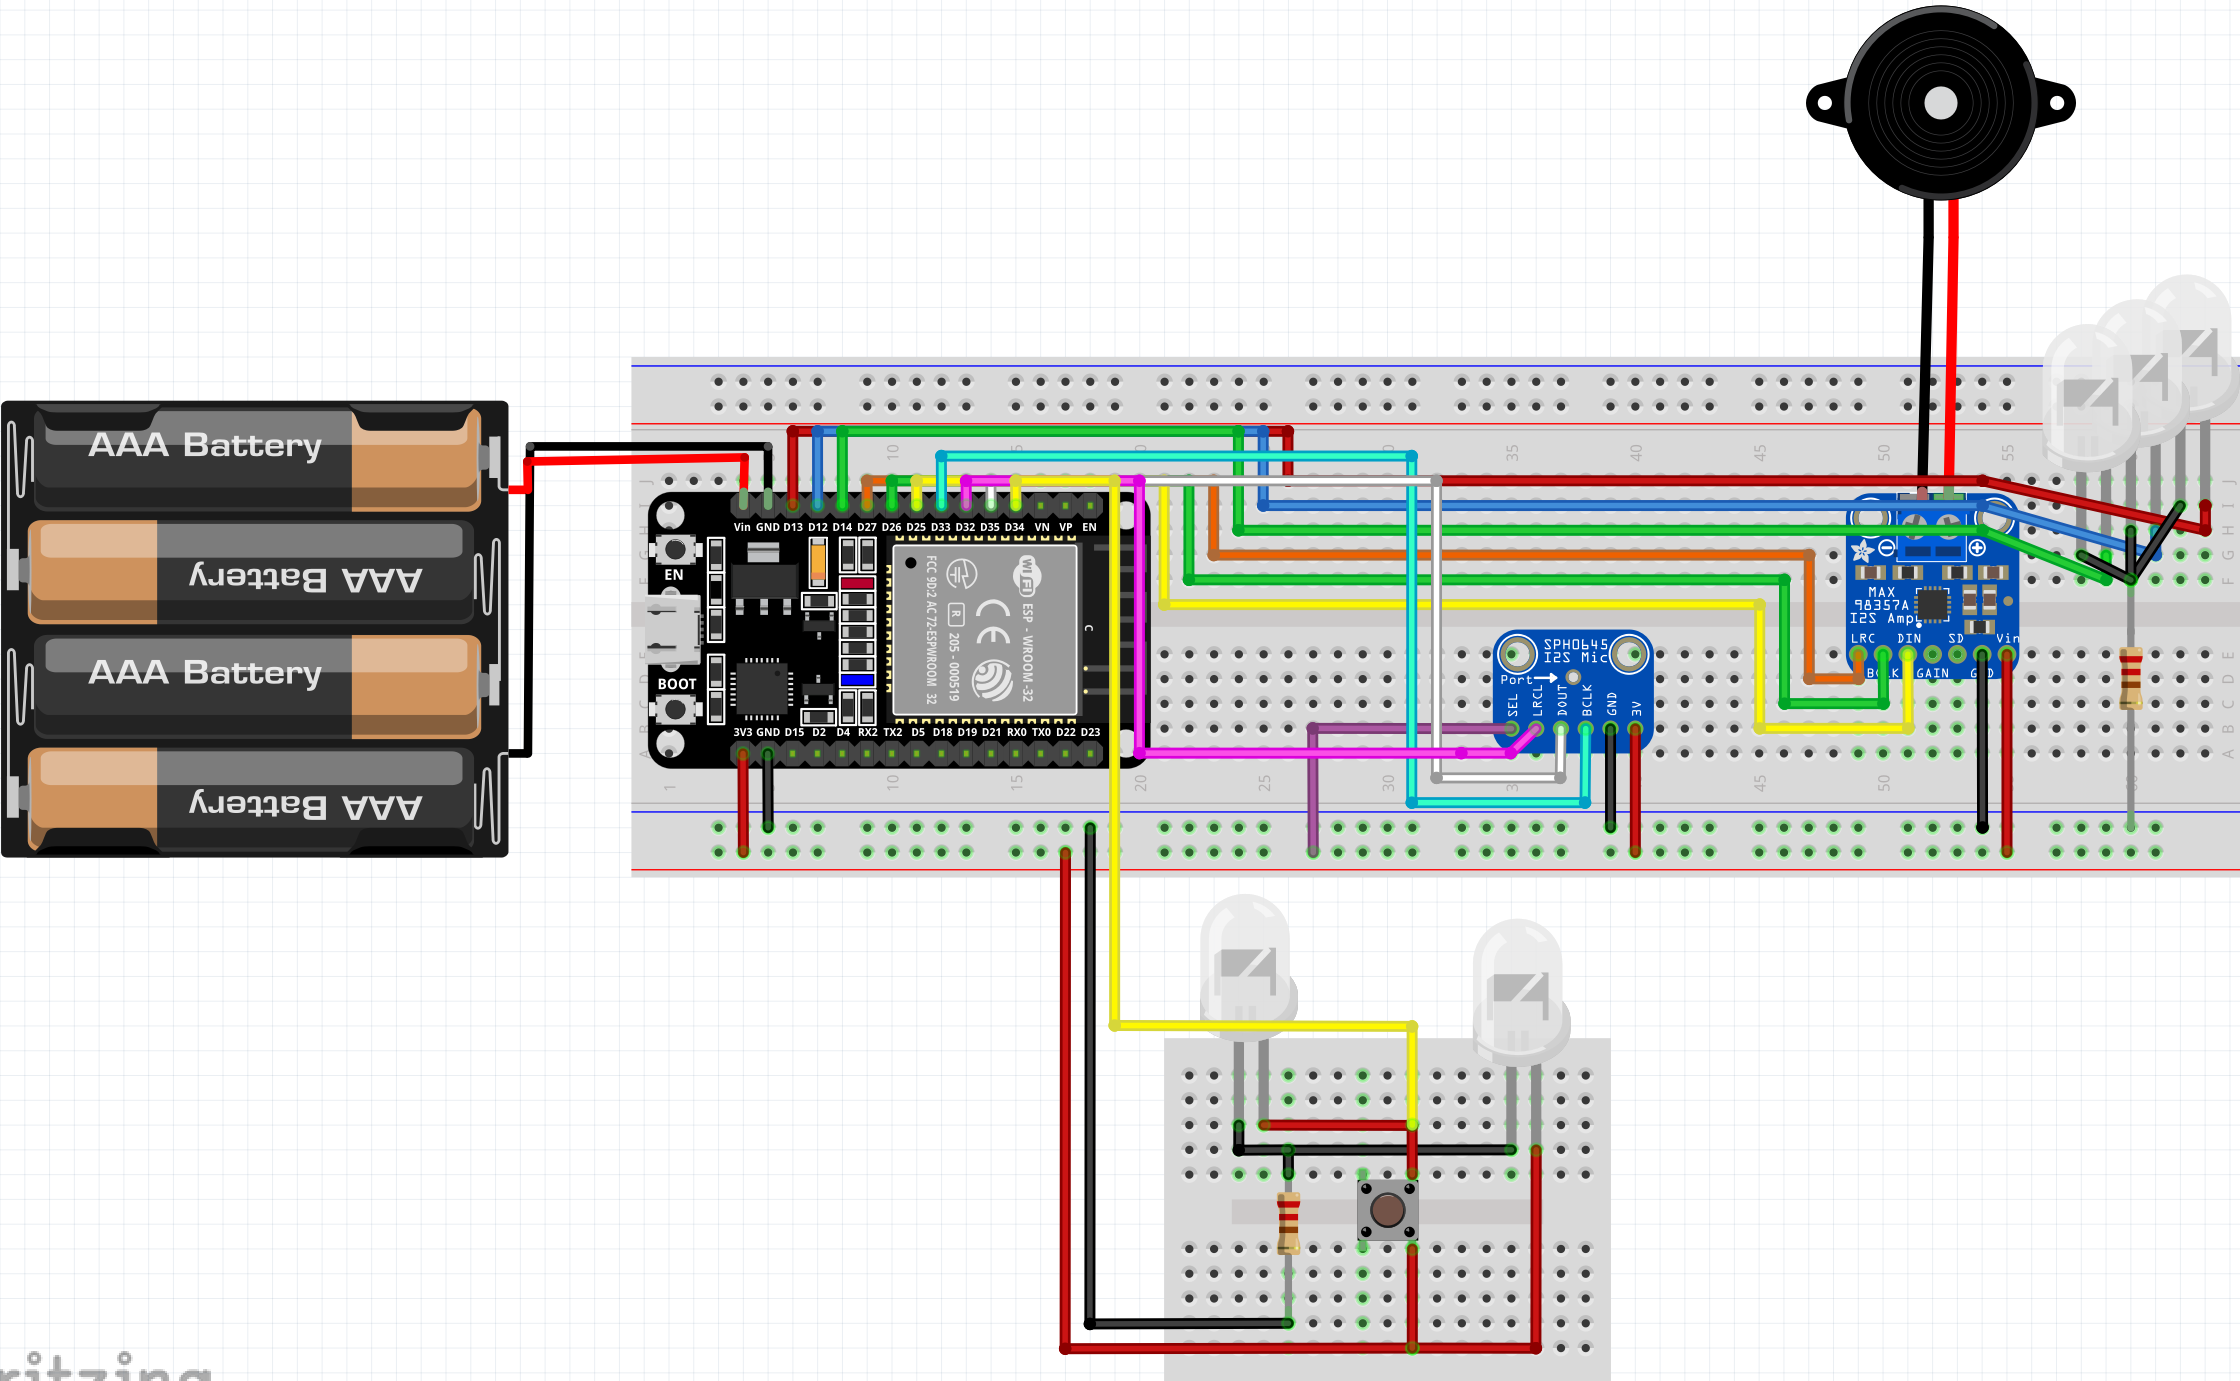
\includegraphics[width=\textwidth]{board_completa.png}
  \caption{Schema del circuito completo con ESP32, microfono I²S, amplificatore MAX98357A, LED di stato e pulsante di hotspot.}
  \label{fig:board_completa}
\end{figure}

\subsection{Realizzazione del PCB}
\label{subsec:pcb_completo}

Dopo aver completato lo schema su breadboard, il progetto è stato trasferito in \textbf{vista PCB} 
all’interno di Fritzing, con le dovute modifiche, ottenendo così una scheda stampata ordinata e compatta, come mostrato in \autoref{fig:pcb_completo}.\\ 
In questa configurazione l’\textbf{ESP32} rimane al centro della scheda, con le piste di segnale distribuite verso i moduli periferici: 
i LED di stato con le relative resistenze sono disposti lungo il bordo destro per facilitare la visibilità [LED-1-2-3], mentre il pulsante di hotspot 
è collocato nella parte inferiore [S2] insieme al LED [LED4] che ne segnala l’attivazione. \\
Il layout delle piste è stato ottimizzato per ridurre le interferenze e mantenere separati i percorsi di potenza da quelli di segnale.\\
Questo passaggio è stato fatto per poter permettere una futura produzione in serie del dispositivo.

\begin{figure}[H]
  \centering
  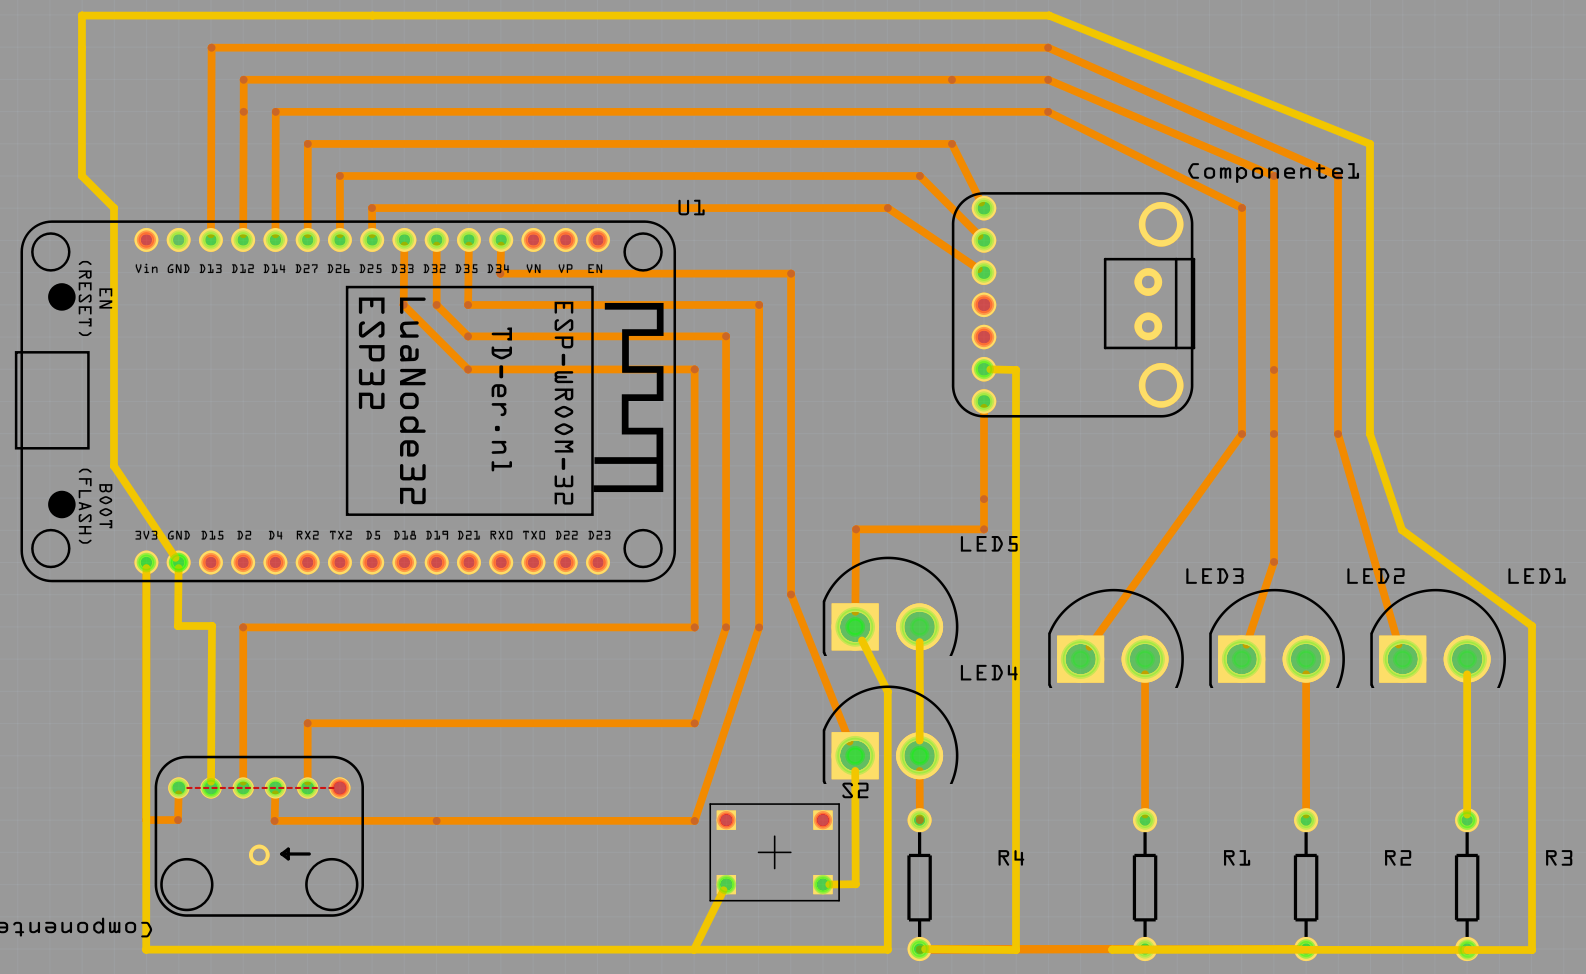
\includegraphics[width=\textwidth]{pcb_completo.png}
  \caption{Layout del circuito stampato (PCB), con ESP32, LED di stato, pulsante di hotspot e connettori di alimentazione.}
  \label{fig:pcb_completo}
\end{figure}
